\documentclass[11pt]{article}
\usepackage[a4paper,margin=1in]{geometry}
\usepackage[T1]{fontenc}
\usepackage[utf8]{inputenc}
\usepackage{lmodern}
\usepackage{microtype}
\usepackage{booktabs}
\usepackage{tabularx}
\usepackage{graphicx}
\usepackage{enumitem}
\usepackage{caption}
\usepackage{xcolor}
\usepackage[colorlinks=true,linkcolor=black,urlcolor=blue!55!black,citecolor=black]{hyperref}
\setlist{itemsep=2pt,topsep=4pt,parsep=0pt}
\captionsetup{font=small,labelfont=bf}
\setlength{\parskip}{5pt}
\setlength{\parindent}{0pt}
\newcommand{\crux}{Crux}

\title{\textbf{Always Medium: Self-Stress-Testing Improves the Wording of AI Decision Briefs but Erases the Confidence Signal}}
\author{Mia (GitHub: Mhiah)\\ \small Independent}
\date{\small AI $\times$ Epistemics Research Sprint, 13--15 November 2026\\ Track 3: Epistemic Products}

\begin{document}
\maketitle
\vspace{-1.2em}

\begin{abstract}
\noindent
A popular fix for overconfident AI advice is to make the system argue against its own answer before it commits. This study tests whether that step produces more honest decision briefs. Nine business decision questions, split into well-evidenced, contested and thin-evidence groups, were answered three ways by the same model: a plain single prompt, a single prompt over retrieved evidence, and a full pipeline that forms a thesis, stress-tests it, re-judges each assumption and then concludes. The last two methods received identical evidence, so the stress test is the only difference between them. Two results pull in opposite directions. Scored blind against a rubric fixed in advance, stress-tested briefs rated highest (23.4 of 25, against 21.8 for one-shot and 16.0 for plain) and were never flagged as overselling. Yet the stress-tested pipeline reported \emph{medium} confidence on all nine questions and judged its own first answer \emph{weakened} all nine times. Its first answer, before the stress test, was high on well-evidenced questions and medium on thin ones; afterwards the label no longer varied at all. No method used \emph{low} in any of 36 confidence labels. On this small sample, self-critique improved how the brief was written while removing the information in its confidence label. A critic that always wins tells the reader nothing, and a rubric that rewards hedged prose cannot see the loss. Stress-test designs need an outcome in which the answer survives.
\end{abstract}

\section{Introduction}

People increasingly ask AI systems what to do: whether to enter a market, change a price, adopt a policy. The reply usually comes as a short brief with a recommendation and a stated level of confidence. The failure this study cares about is not that such briefs are wrong. It is that they can sound equally sure whether the evidence behind them is strong, mixed or nearly absent, which leaves the reader unable to tell a well-supported recommendation from a guess.

One widely used remedy is self-critique: have the system commit to an answer, search for what would prove it wrong, and only then write the brief. The idea appears in debate and verification methods \cite{du2023debate,dhuliawala2023cove} and in product sketches of AI advisers that challenge the user's and their own reasoning \cite{forethought_angels}. It is intuitive, and it makes for good demonstrations, because the output visibly contains doubts and counter-arguments.

The open question is whether the extra step changes the epistemic content of the brief or only its tone. A brief can list caveats and still tell the reader nothing about how much to rely on it. This study separates the two by measuring:

\begin{enumerate}
\item whether a brief's stated confidence follows the strength of the evidence, counted directly from the confidence labels with no human or model judgement involved;
\item whether the brief is better by a rubric fixed before any brief was generated;
\item what the stress test does to the answer it is applied to.
\end{enumerate}

\textbf{Contributions.} (i) A controlled comparison in which the stress-tested and one-shot methods see identical evidence, which isolates the effect of the stress test. (ii) A judgement-free measure of whether confidence tracks evidence, built from three evidence groups. (iii) An observation that the two measures disagree: the stress test raised rubric scores while flattening the confidence label to a single value. (iv) An open harness, question set, rubric and full run records, so the result can be checked and extended.

\section{Related Work}

\textbf{Verbalised confidence.} Language models can be asked to state their confidence in words, and such statements are often poorly calibrated and skewed towards overconfidence \cite{xiong2024uncertainty}. This study does not measure calibration against ground truth; it measures the weaker property of whether confidence varies with evidence at all.

\textbf{Self-critique and debate.} Multi-agent debate \cite{du2023debate} and chain-of-verification \cite{dhuliawala2023cove} report gains in factual accuracy from having a model check or contest a draft answer. Those evaluations use questions with known answers. Decision questions rarely have one, so the effect of self-critique on stated confidence has to be examined separately.

\textbf{Sycophancy.} Models tend to shift towards what a user appears to believe \cite{sharma2023sycophancy}, and sycophantic advice has measurable effects on the people who receive it \cite{science_sycophancy}. The pattern reported here is related but distinct: a model yielding to a critic that it generated itself.

\textbf{Epistemic products.} Forethought's ``angels on the shoulder'' sketches describe AI advisers whose value depends on advice the user would later endorse \cite{forethought_angels}. The Habermas Machine drafts group statements that find common ground \cite{tessler2024habermas}. The sprint's Track 3 asks for rubrics that grade decision briefings; this study contributes one, and reports a way in which such a rubric can mislead.

\section{Methodology}

\subsection{System under test}

The stress-tested method is \crux{} \cite{crux}, a research engine written by the author before the sprint. For a question it (1) plans web searches, about half aimed at evidence against a ``yes'' answer; (2) collects up to 20 sources and extracts factual claims, discarding any claim whose quoted passage cannot be found in its source; (3) forms a \emph{thesis} with a confidence label and explicit assumptions; (4) runs a \emph{stress test} that attacks every assumption; (5) \emph{re-evaluates} each assumption as supported, weakened, contradicted or unresolved and gives the thesis an overall verdict of strengthened, survived, weakened or overturned; and (6) writes a \emph{conclusion} with a new confidence label. Confidence is one of \emph{low}, \emph{medium} or \emph{high} at every stage. \crux{} was used unchanged at a fixed commit (\texttt{359a6f4}).

\subsection{Three methods, one model}

For each question the harness produced three briefs:

\begin{itemize}
\item \textbf{Plain.} One prompt asking for a decision brief. No web evidence.
\item \textbf{One-shot.} One neutral prompt over the claims \crux{} extracted for that question.
\item \textbf{Stress-tested.} \crux{}'s final conclusion.
\end{itemize}

One-shot and stress-tested briefs are built from exactly the same claims in the same run, so the only difference is the thesis, stress-test and re-evaluation stages. Comparing plain with one-shot shows what evidence alone adds. All three briefs share one output schema: an answer, a confidence label with a rationale, open uncertainties and next steps; the two evidence-based methods also cite claims. \crux{}'s own first answer (the thesis) was recorded as a fourth data point for confidence only.

All calls used \texttt{gpt-5.4-mini} (2026-03-17 snapshot) through SERV Reasoning at temperature 0.2, with Tavily advanced search. Each question took 8 model calls and up to 12 searches. The harness refuses to run without live API keys, so no sample data can enter the results.

\subsection{Questions}

Nine yes/no business questions were written before any run and assigned by the author to three groups of three (Appendix~\ref{app:questions}):

\begin{itemize}
\item \textbf{Well-evidenced:} substantial public data points one way (for example, whether a consumer app in Nigeria should be built for mobile first).
\item \textbf{Contested:} serious evidence on both sides (for example, a four-day work week).
\item \textbf{Thin evidence:} a niche so specific that little direct evidence should exist (for example, cultivated-meat pet food subscriptions in Kenya).
\end{itemize}

A method whose confidence means anything should, on average, be less sure in the thin-evidence group than in the well-evidenced group.

\subsection{Measures}

\textbf{Confidence labels.} Read directly from the saved output of each method. No scoring is involved.

\textbf{Rubric.} Each of the 27 briefs was scored from 1 to 5 on five criteria: honest confidence, counter-evidence, traceability, cruxes and useful next steps, plus a yes/no flag for overselling (Appendix~\ref{app:rubric}). The rubric was committed to the public repository before the first brief was generated.

\textbf{Scoring procedure.} Briefs were rendered in one uniform layout, stripped of inline citation marks, shuffled and given random identifiers. They were scored by an AI model (Claude, Anthropic), a different model family from the one that wrote the briefs. The key was applied only after all scores were recorded. Section~\ref{sec:limits} lists the ways in which this blinding was imperfect.

\textbf{Stress-test record.} For the stress-tested method, the verdict on the thesis, the verdict on each assumption, and the type and severity of each challenge were counted from the run records.

\section{Results}

\subsection{The confidence label stops varying after the stress test}

Figure~\ref{fig:labels} shows every confidence label. Three things stand out.

\begin{figure}[t]
\centering
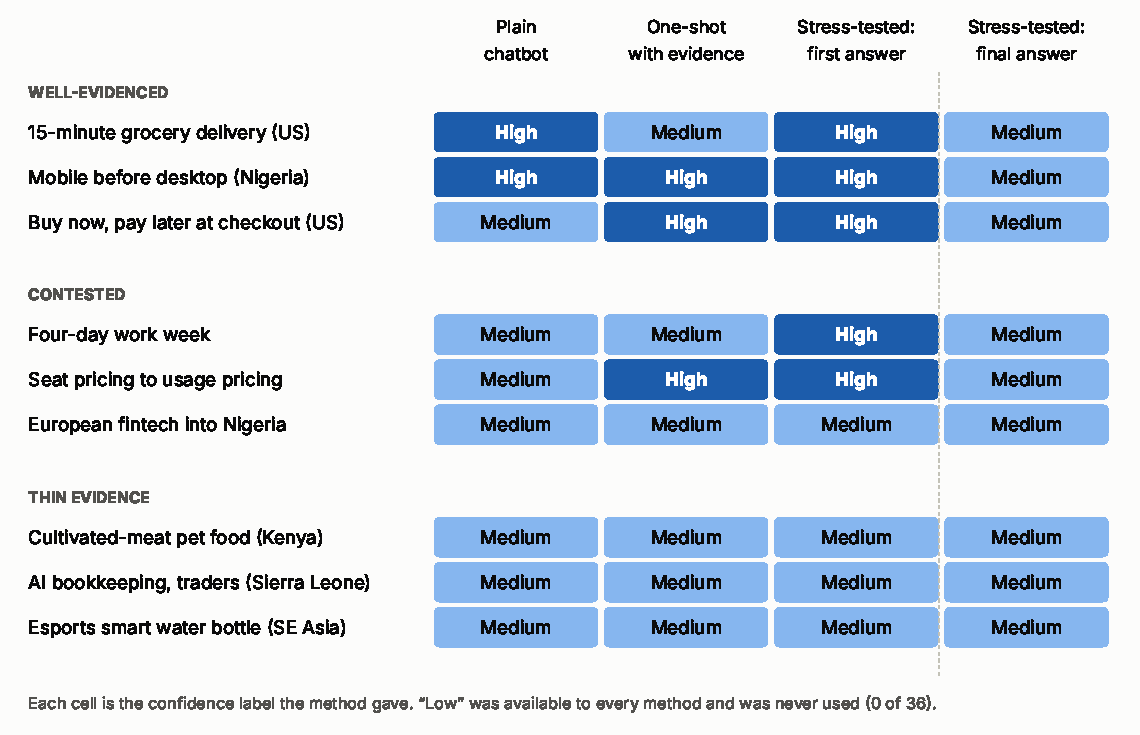
\includegraphics[width=0.92\linewidth]{figure1.pdf}
\caption{The confidence label each method gave for each question. The right-hand column is the same pipeline as the column to its left, after the stress test.}
\label{fig:labels}
\end{figure}

First, the stress-tested pipeline ended on \emph{medium} for all nine questions. Its label has no variance, so it cannot distinguish a well-evidenced question from a thin one.

Second, the same pipeline's first answer did vary, and in the expected direction: high on all three well-evidenced questions, high on two of three contested ones, medium on all three thin-evidence ones. Table~\ref{tab:tier} gives the group means. The first answer shows the steepest drop from well-evidenced to thin; the one-shot brief shows a smaller drop; the stress-tested final answer shows none.

Third, no method ever said \emph{low}. Across 36 labels there were 10 \emph{high}, 26 \emph{medium} and 0 \emph{low}, including on the three questions chosen because direct evidence should be scarce. The three-level scale was used as a two-level one, and the stress test reduced it to one level.

\begin{table}[h]
\centering
\small
\begin{tabular}{lcccc}
\toprule
 & Well-evidenced & Contested & Thin evidence & Labels used \\
\midrule
Plain & 2.67 & 2.00 & 2.00 & 2 high, 7 medium \\
One-shot with evidence & 2.67 & 2.33 & 2.00 & 3 high, 6 medium \\
Stress-tested: first answer & 3.00 & 2.67 & 2.00 & 5 high, 4 medium \\
Stress-tested: final answer & 2.00 & 2.00 & 2.00 & 9 medium \\
\bottomrule
\end{tabular}
\caption{Mean confidence by evidence group (low = 1, medium = 2, high = 3; three questions per group).}
\label{tab:tier}
\end{table}

\subsection{The stress test always won}

The pipeline can return four verdicts on its first answer: strengthened, survived, weakened or overturned. It returned \emph{weakened} in 9 of 9 runs. Where the first answer was high (5 runs), confidence fell to medium; where it was already medium (4 runs), it stayed there.

The stress test raised 68 challenges (7.6 per question), and 67 of them were rated major or critical. Only 8 were contradictory evidence. The rest were weak assumptions (18), alternative explanations (15), missing evidence (15) and risks (12): objections that can be raised against almost any recommendation, whatever the evidence. Of 43 assumptions judged, 31 were weakened, 7 unresolved, 5 supported and none contradicted.

The mobile-first question shows the mechanism. Plain, one-shot and first-answer briefs all said \emph{high}; the evidence on mobile use in Nigeria was consistent across official, industry and research sources. The stress test objected that the evidence did not identify ``the startup's actual target segment'' or compare mobile-first with desktop-first launches. Both points are true, and neither could be answered by any evidence, because the question names no particular startup. The final brief dropped to \emph{medium}. The confidence fell because of what the question left open, not because of anything found.

\subsection{Stress-tested briefs scored highest on the rubric}

Table~\ref{tab:rubric} gives the blind rubric scores. Stress-tested briefs scored highest overall, highest or joint highest on four of five criteria, and none was flagged as overselling. Against the one-shot brief on the same question and the same evidence, the stress-tested brief had the higher total in 7 of 9 questions and tied in 2.

\begin{table}[h]
\centering
\small
\begin{tabular}{lccccccc}
\toprule
 & Honest & Counter- & Trace- & & Next & Total & Flagged \\
 & confidence & evidence & ability & Cruxes & steps & (of 25) & oversold \\
\midrule
Plain & 3.11 & 2.89 & 1.00 & 4.00 & 5.00 & 16.0 & 2 of 9 \\
One-shot with evidence & 4.00 & 4.00 & 5.00 & 3.89 & 4.89 & 21.8 & 1 of 9 \\
Stress-tested & 4.89 & 4.33 & 4.78 & 4.44 & 5.00 & 23.4 & 0 of 9 \\
\bottomrule
\end{tabular}
\caption{Mean rubric scores (1--5 per criterion, 9 briefs per method), scored blind.}
\label{tab:rubric}
\end{table}

Most of the gap between plain and the other two is traceability: a plain brief cites nothing a reader can check. Evidence alone accounts for 5.8 of the 7.4 points separating plain from stress-tested; the stress test adds a further 1.6. The largest single-criterion gain from the stress test was on honest confidence (4.00 to 4.89). All three briefs flagged as overselling carried a \emph{high} label. The next-steps criterion did not discriminate: nearly every brief scored 5.

\subsection{The two measures disagree}

The stress test's largest rubric gain was on ``honest confidence'', the very property on which its label carried no information. Both results come from the same nine briefs. The rubric criterion asks whether the stated confidence matches the support \emph{the brief itself shows}. A brief that says \emph{medium} and lists what is missing satisfies that criterion on every question, whether evidence was abundant or scarce. Reading one brief at a time, a scorer has no way to notice that the label never changes; that only appears across the set.

\section{Discussion}

\textbf{A critic that cannot lose is not informative.} The stress-test stage is told to find what could make the thesis wrong and to attack every assumption. For a general decision question, some assumption can always be attacked and some evidence is always missing. The re-evaluation stage then finds the thesis dented, every time. The outcome is predictable before the run, so it tells the reader nothing about this question in particular. In these runs the first answer carried more information about evidence strength than the final one did.

\textbf{This is not a claim that medium was the wrong label.} There is no ground truth here. On the thin-evidence questions, \emph{medium} confidence in a cautious ``pilot first'' answer may be reasonable. The finding is narrower: a label that is the same for every question cannot help a reader decide which briefs to rely on, and the stress test is what made it the same.

\textbf{Rubrics can reward the appearance of calibration.} Per-brief rubric scoring, by a person or a model, favours text that hedges and names its gaps. That is worth something: stress-tested briefs did surface more counter-evidence and sharper conditions. But it means a pipeline can raise its rubric score on honesty while its confidence signal degrades. Evaluations of epistemic products should include a set-level check, such as the one used here, alongside per-item scoring.

\textbf{Design implications.} These follow from the mechanism and were not tested here:
\begin{itemize}
\item Give the critic a way to lose. Count a challenge against the thesis only when it is backed by evidence in the record, and treat ``this evidence is missing'' separately from ``this evidence contradicts''. Only 8 of 68 challenges here were contradictory evidence.
\item Separate what the question leaves open from what the evidence leaves open. Unknowns that no research could resolve belong in the conditions of the answer, not in a lower confidence label.
\item Report the first and final confidence together. \crux{} already records both; the pair is more informative than either alone.
\item Test any confidence scale on questions designed to be thin. A scale whose lowest level is never used on such questions is not doing its job.
\end{itemize}

\textbf{What would change this conclusion.} The pattern could be specific to this model, this prompt wording, the three-level scale or business questions. It could also soften with more questions: nine runs returning the same verdict is striking, but a tenth could differ. The run records and harness are public so that others can check \cite{vet}.

\section{Conclusion}

On nine decision questions, making an AI system stress-test its own answer produced briefs that scored higher on a rubric fixed in advance and were never flagged as overselling. It also produced the same confidence label and the same verdict on every question, removing the variation that the system's first answer had shown between well-evidenced and thin-evidence questions. Self-critique changed how the briefs were worded more than it changed what a reader could learn from their confidence. For builders of AI advisers, the practical point is that a self-critique step should be evaluated on whether its outcome ever differs, not only on whether its output reads as careful.

\begin{thebibliography}{9}\small
\bibitem{du2023debate} Y. Du, S. Li, A. Torralba, J. B. Tenenbaum and I. Mordatch. Improving Factuality and Reasoning in Language Models through Multiagent Debate. arXiv:2305.14325, 2023.
\bibitem{dhuliawala2023cove} S. Dhuliawala et al. Chain-of-Verification Reduces Hallucination in Large Language Models. arXiv:2309.11495, 2023.
\bibitem{xiong2024uncertainty} M. Xiong et al. Can LLMs Express Their Uncertainty? An Empirical Evaluation of Confidence Elicitation in LLMs. ICLR, 2024.
\bibitem{sharma2023sycophancy} M. Sharma et al. Towards Understanding Sycophancy in Language Models. arXiv:2310.13548, 2023.
\bibitem{science_sycophancy} Sycophantic AI Decreases Prosocial Intentions and Promotes Dependence. \emph{Science}. \url{https://www.science.org/doi/10.1126/science.aec8352}
\bibitem{tessler2024habermas} M. H. Tessler et al. AI Can Help Humans Find Common Ground in Democratic Deliberation. \emph{Science}, 2024. \url{https://www.science.org/doi/10.1126/science.adq2852}
\bibitem{forethought_angels} Forethought. Design Sketches: Angels-on-the-Shoulder. \url{https://www.forethought.org/research/design-sketches-angels-on-the-shoulder}
\bibitem{crux} Crux (pre-existing system under test), commit \texttt{359a6f4}. \url{https://github.com/Mhiah/crux}
\bibitem{vet} Vet: harness, questions, rubric, run records and analysis for this study. \url{https://github.com/Mhiah/Vet}
\end{thebibliography}

\appendix

\section{Limitations and Dual-Use / Ethical Considerations}
\label{sec:limits}

\subsection*{Limitations}

\begin{itemize}
\item \textbf{Small sample, single runs.} Nine questions, one run each, at temperature 0.2. No confidence intervals are reported because none would be meaningful. The results indicate a pattern to test, not an effect size.
\item \textbf{One model, one pipeline, one domain.} Every brief came from one model through one provider, the stress test is one implementation with one set of prompts, and all questions are business decisions. The flattening may not appear with other models, prompts, finer confidence scales or domains.
\item \textbf{Prompt asymmetry.} \crux{}'s thesis stage is told to commit to a clear position rather than hedge. Some of the drop from first to final answer may reflect that instruction as well as the stress test. The one-shot method, which has a neutral prompt and the same evidence, is the cleaner comparison, and it also varied by evidence group where the final answer did not.
\item \textbf{Evidence groups are the author's judgement.} Questions were assigned to groups before the runs, without an independent panel. Retrieval returned 20 sources for every question, including the thin-evidence ones, where the evidence was mostly indirect.
\item \textbf{The rubric has no expert panel.} It was written by the author. One criterion (next steps) hit the ceiling and did not discriminate.
\item \textbf{Scoring by a single AI model, with imperfect blinding.} All rubric scores come from one pass by one AI model; there is no second scorer and no human check, so scorer reliability is unknown. Plain briefs cite no evidence and are therefore identifiable. The scoring model had also seen the confidence labels in the run log before scoring, and the same AI assistant helped write the harness. The rubric results should be treated as indicative. The confidence-label and stress-test results do not depend on scoring.
\item \textbf{No ground truth.} The study measures whether briefs are honest about their support, not whether their recommendations are correct.
\item \textbf{The author built the system under test.} The headline finding is unfavourable to that system, but the conflict of interest is real and the data are public for that reason.
\end{itemize}

\subsection*{Dual-use and ethical considerations}

\begin{itemize}
\item \textbf{Honesty theatre.} The main risk this work points to is a product that looks rigorous without being informative. A visible ``we stress-tested this'' step, with listed doubts and an even-handed tone, may raise user trust while the confidence signal carries nothing. The rubric here could be used to tune briefs for that appearance. The set-level check in Section~4.1 is the proposed safeguard.
\item \textbf{Persuasion.} Knowing which features make a brief read as careful could help someone make weak advice more convincing. The features involved (hedged confidence, listed caveats) are already well known, so the marginal uplift is small.
\item \textbf{Over-reading the result.} The opposite misuse is to cite this study as evidence that self-critique is useless. It is not: stress-tested briefs surfaced more counter-evidence and clearer conditions. The claim is about the confidence label.
\item \textbf{Data.} No personal data or human participants were involved. All evidence came from public web pages, and every extracted claim is stored with its source.
\end{itemize}

\subsection*{Prior work and AI assistance}

\crux{} was written before the sprint and is used unchanged. Everything in the Vet repository was produced during the sprint: the question set, the harness, the plain and one-shot comparison methods, the rubric, the run records, the analysis and this report. An AI assistant (Claude, Anthropic) was used to write the harness and analysis code, to score the briefs as described, and to help draft this report. The author is responsible for all content. Every number in the report is computed by \texttt{analysis/analyze.py} from files in the repository.

\section{Questions}
\label{app:questions}

\small
\begin{tabularx}{\linewidth}{llX}
\toprule
ID & Group & Question \\
\midrule
W1 & Well-evidenced & Should a US startup launch a 15-minute ultrafast grocery delivery service in 2026? \\
W2 & Well-evidenced & Should a new consumer app startup in Nigeria build for mobile before desktop web? \\
W3 & Well-evidenced & Should a small online retailer in the US offer buy now, pay later at checkout to increase sales? \\
C1 & Contested & Should a mid-sized software company adopt a four-day work week? \\
C2 & Contested & Should a B2B SaaS startup switch from per-seat pricing to usage-based pricing? \\
C3 & Contested & Should a European fintech company expand into Nigeria in 2026? \\
T1 & Thin evidence & Should a startup launch a subscription service for cultivated-meat pet food in Kenya? \\
T2 & Thin evidence & Should a startup sell a paid AI bookkeeping tool to market traders in Sierra Leone? \\
T3 & Thin evidence & Should a hardware startup launch a smart water bottle for competitive esports players in Southeast Asia? \\
\bottomrule
\end{tabularx}

\normalsize
Twelve questions were written; nine were run, three per group, because of API budget. The three not run (one per group) are in \texttt{questions.json} and have no results.

\section{Rubric}
\label{app:rubric}

\small
\begin{tabularx}{\linewidth}{lX}
\toprule
Criterion & What a score of 5 requires \\
\midrule
Honest confidence & Confidence is clearly tied to how strong and complete the support shown in the brief is, including what is missing. \\
Counter-evidence & States the strongest case against its own answer and says how it changes the answer. \\
Traceability & Every load-bearing claim points to specific evidence a reader could look up. \\
Cruxes & Names the specific, testable conditions that would flip the answer. \\
Useful next steps & Concrete, cheap steps, each tied to the uncertainty it would resolve. \\
Oversold (yes/no) & The answer states something more strongly than the support in the brief allows. \\
\bottomrule
\end{tabularx}

\normalsize
The full rubric with anchors for scores 1, 3 and 5 is in \texttt{rubric.md}.

\end{document}
